\documentclass[11pt,a4paper]{article}
\usepackage[T1]{fontenc}
\usepackage[utf8]{inputenc}
\usepackage[magyar]{babel}
\usepackage[margin=2.5cm]{geometry}
\usepackage{amsmath}
\usepackage{graphicx}
\usepackage{pdflscape}
\usepackage{booktabs}
\usepackage{float}
\usepackage{caption}
\captionsetup{font=small}

\title{3D HP-hajtogatás evolúciós algoritmussal:\\a mutáció helyének hatása}
\author{Nágó Dániel}
\date{Bioinformatikai Algoritmusok \\ Sapientia EMTE, Marosvásárhely}

\begin{document}
\maketitle

\begin{abstract}
\noindent A dolgozat a HP-modell 3D hajtogatási feladatát genetikus algoritmussal
(GA) oldja meg. Azt vizsgáljuk, hogy a mutáció helye a lépéssorozatban
befolyásolja-e az algoritmus sikerét és futásidejét. Nyolc mutációs profilt
hasonlítunk össze öt szekvencián, 2D és 3D rácson, profilonként 30 független
futással. A profilok között a Holm-korrekciót kibíró eltérést nem találtunk,
kivéve, hogy a túl meredeken növekvő \texttt{tail\_exp} profil a 2D hosszú
láncoknál rosszabb energiát ad. A 3D hajtogatás minden vizsgált szekvencián
szignifikánsan alacsonyabb energiát ér el, mint a 2D. A populáció változatossága
minden profilnál az első 100 generációban a kezdeti érték harmadára vagy kisebbre
esik. Feltáró mérésben a mutációs ráta növelése rontott az eredményen, a véletlen
új egyedek beillesztése a 36 aminosavas láncon javulást mutatott, ez azonban 30
futással nem szignifikáns.
\end{abstract}

\section{A probléma}

A fehérjék aminosav-láncok, amelyek vízben meghatározott térszerkezetbe
hajtogatódnak. A HP-modellben minden aminosav hidrofób (H) vagy poláris (P).
A lánc egy rács pontjain helyezkedik el, 2D-ben négyzetrácson, 3D-ben
kockarácson, és két aminosav nem foglalhatja el ugyanazt a pontot. Az energia
minden olyan H-H párra $-1$, amely a rácson szomszédos, a láncban azonban nem. A
cél a legkisebb energiájú hajtogatás megtalálása. A feladat NP-nehéz, ezért
genetikus algoritmust (GA) alkalmazunk.

Egy megoldás $n-2$ relatív lépésből álló sztring: előre, balra, jobbra, fel vagy
le (2D-ben csak az első három). Az első kötés rögzített. Egy korai lépés
megváltoztatása a lánc hátralévő részét elforgatja, egy késői lépés csak a lánc
végét mozdítja el.

\section{Kutatási kérdések}

\paragraph{Fő kérdés.} Hogyan függ a GA eredménye és futásideje attól, hogy a
lépéssorozat melyik pozícióit mutáljuk? Futásidőn az optimum eléréséhez szükséges
kiértékelések számát, eredményen a sikerarányt és a végső energiát értjük. A
vizsgálat arra irányul, hogy javít-e az eredményen, ha a lánc végéhez közeli
lépéseket nagyobb valószínűséggel mutáljuk. Adaptív változatokat is vizsgálunk, amelyekben
az eloszlás a futás során módosul.

\paragraph{Másodlagos kérdés.} Több H-H kapcsolatot ér-e el a 3D változat, mint
a 2D?

\section{Hipotézisek}

A négy hipotézis szövege a végső mérés előtt készült, és azóta nem változott. A
hipotézisek rögzítése után három adaptív profil (\texttt{adaptive\_rev},
\texttt{adaptive\_exp}, \texttt{adaptive\_exp\_rev}) került a vizsgálatba, ezért
ezek eredményét feltáró jellegűnek tekintjük. A profilokat a Módszer fejezet
írja le.

\begin{description}
\item[H1] A vég felé növekvő profilok az egyenletesnél kevesebb kiértékelésből és
kevesebb generációból érik el a célenergiát, és a végső energiájuk nem rosszabb.
\item[H2] A fordított profil rosszabb az egyenletesnél.
\item[H3] Az adaptív profil, amely a vég felé növekvő profilról fokozatosan
egyenletesre vált, legalább olyan jó, mint a legjobb fix profil.
\item[H4] A 3D változat ugyanazon a szekvencián több H-H kapcsolatot ér el, mint a
2D.
\end{description}

Az eredeti döntési szabály szerint egy hipotézist akkor tekintünk igazoltnak, ha
legalább 30 független futás után a Mann-Whitney-próba $p<0{,}05$ értéket ad, és az
eltérés iránya megegyezik a várttal. A vizsgálat sok összehasonlítást tartalmaz,
ezért a szabályt a mérés után kiegészítettük: a Holm-korrekcióval módosított
$p$-értéknek is 0,05 alatt kell maradnia. Mindkét értéket közöljük.

\section{Módszer}

\paragraph{A genetikus algoritmus.} A populáció 200 egyedből áll. A szelekció
háromegyedes versenyszelekció, a keresztezés egypontos, 0,9 valószínűséggel. A
két legjobb egyed változatlanul kerül a következő generációba. A mutáció minden
lépést külön, saját valószínűséggel módosít. Az érvénytelen hajtogatás (két aminosav ugyanazon a ponton)
ütközésenként 5 büntetőpontot kap. A futás leáll, ha eléri a célenergiát. Egy
generáció 198 új egyedet értékel ki, ezért a kiértékelések száma $200+198g$, ahol
$g$ a generációk száma. A kettő így gyakorlatilag ugyanazt méri, ezért az
eredményekben csak a kiértékeléseket közöljük.

\paragraph{A nyolc mutációs profil.} Minden profil azonos, $1/(n-2)$ átlagos
rátával dolgozik, csak az eloszlás alakja különbözik.
\begin{itemize}
\item \texttt{uniform}: minden lépés azonos eséllyel mutál.
\item \texttt{tail}: a mutáció esélye a lánc vége felé lineárisan nő.
\item \texttt{tail\_exp}: az esély $1{,}2^i$ szerint nő, ahol $i$ a lépés sorszáma.
\item \texttt{head}: a \texttt{tail} tükörképe, az esély az eleje felé nő.
\item \texttt{adaptive}: a futás elején \texttt{tail}, amely a generációk során
lineárisan átmegy \texttt{uniform}-ba. Az \texttt{adaptive\_exp} ugyanez
\texttt{tail\_exp}-pel.
\item \texttt{adaptive\_rev}: a futás elején \texttt{uniform}, amely a futás
végére \texttt{tail}-lé alakul. Exponenciális párja az
\texttt{adaptive\_exp\_rev}, amely \texttt{tail\_exp}-be vált.
\end{itemize}
Az $1{,}2$ alapot előzetes mérésben választottuk az $1{,}1$, $1{,}2$ és $1{,}3$
közül.

\paragraph{Szekvenciák és célenergiák.} Öt szekvenciát vizsgálunk mindkét
rácson: három rövidet (20, 24 és 25 aminosav) és két hosszabbat (36 és 48
aminosav). Siker alatt a célenergia elérését értjük.

\begin{center}
\footnotesize
\begin{tabular}{rlrr}
\toprule
$n$ & szekvencia & 2D cél & 3D cél \\
\midrule
20 & \texttt{HPHPPHHPHPPHPHHPPHPH} & $-9$ & $-11$ \\
24 & \texttt{HHPPHPPHPPHPPHPPHPPHPPHH} & $-9$ & $-13$ \\
25 & \texttt{PPHPPHHPPPPHHPPPPHHPPPPHH} & $-8$ & $-9$ \\
36 & \texttt{PPPHHPPHHPPPPPHHHHHHHPPHHPPPPHHPPHPP} & $-14$ & $-18$ \\
48 & \texttt{PPHPPHHPPHHPPPPPHHHHHHHHHHPPPPPPHHPPHHPPHPPHHHHH} & $-23$ & $-31$ \\
\bottomrule
\end{tabular}
\end{center}

A 2D célok és a 36, illetve 48 aminosavas láncok 3D céljai az irodalomban
ismert legjobb értékek (arXiv 2105.13226). A 3D $-11$, $-13$ és $-9$
célenergiát saját pontos számítással optimálisnak igazoltuk.

\paragraph{Mérés.} A végső mérés 8 profilból, 5 szekvenciából, 2 rácsból és 30
magból áll, összesen 2400 futásból. A magok 0-tól 29-ig számozottak. A rövid szekvenciáknál a keret 300 generáció (59\,600
kiértékelés). A hosszabb láncoknál 1500 generációra (297\,200 kiértékelés)
emeltük, mert az előzetes mérésben 300 generációval szinte sosem találtunk
megoldást.

\paragraph{Statisztika.} Minden profilt az egyenletessel hasonlítunk össze,
ugyanazon rács és szekvencia mellett. A kiértékelések számát és az energiát
Mann-Whitney-próbával, a sikerek számát Fisher-próbával vizsgáljuk. A sikertelen futás a teljes keretet felhasználta, ezért
ennyi kiértékeléssel szerepel az elemzésben. Az ERT (várható futásidő a célig)
az összes futás összes kiértékelése osztva a sikeres futások számával. Ha egy
cellában nincs sikeres futás, az ERT nem értelmezhető.

\paragraph{A populáció változatossága.} A változatosságot a populáció
lépéssorozatai közötti átlagos páronkénti Hamming-távolsággal mérjük, elosztva a
sztring hosszával. Értéke 0, ha minden egyed azonos, véletlen populációra pedig
$(k-1)/k$, ahol $k$ a lehetséges lépések száma (2D-ben 0,67, 3D-ben 0,8). A mérés
minden ötödik generációban történik. A GA ilyenkor a célenergia elérésekor sem
áll le, hanem a teljes keretet felhasználja, így az egy cellához tartozó futások
azonos hosszúak. A magok és a beállítások megegyeznek a végső mérésével. Minden profilt az egyenletessel
Mann-Whitney-próbával hasonlítunk össze a futás egészére átlagolt és a végső
változatosságon, összesen 70 próbával, Holm-korrekcióval. A változatosság nem
szerepelt a hipotézisek között, ezért vizsgálata feltáró jellegű.

\section{Eredmények}

\subsection{Sikerarány és ERT}

Az 1. táblázat a célenergiát elérő futások számát adja meg 30 futásból, a 2.
táblázat az ERT-t. Az oszlopok a rácsot (2D, 3D) és a lánc hosszát jelölik, az
első négy sor a fix, az utolsó négy az adaptív profil.

\begin{table}[H]
\centering
\small
\setlength{\tabcolsep}{4pt}
\begin{tabular}{lrrrrrrrrrr}
\hline
profil & 2D 20 & 2D 24 & 2D 25 & 2D 36 & 2D 48 & 3D 20 & 3D 24 & 3D 25 & 3D 36 & 3D 48 \\
\hline
uniform & 15 & 2 & 3 & 0 & 0 & 21 & 7 & 22 & 3 & 0 \\
tail & 11 & 6 & \textbf{9} & \textbf{1} & 0 & 23 & 8 & \textbf{25} & \textbf{8} & 0 \\
tail\_exp & 9 & 6 & 2 & 0 & 0 & 17 & 4 & 20 & 1 & 0 \\
head & 9 & 2 & 3 & 0 & 0 & 21 & \textbf{11} & 17 & 5 & 0 \\
adaptive & \textbf{16} & 3 & 3 & 0 & 0 & 16 & 7 & 16 & 3 & 0 \\
adaptive\_rev & 11 & 7 & 5 & 0 & 0 & 21 & 4 & 23 & \textbf{8} & 0 \\
adaptive\_exp & 13 & \textbf{8} & 6 & 0 & 0 & 20 & 3 & 22 & 3 & 0 \\
adaptive\_exp\_rev & 14 & 5 & \textbf{9} & 0 & 0 & \textbf{24} & 6 & \textbf{25} & 6 & 0 \\
\hline
\end{tabular}

\caption{A célenergiát elérő futások száma 30-ból. Félkövér: a legjobb érték oszloponként.}
\end{table}

\begin{table}[H]
\centering
\small
\setlength{\tabcolsep}{4pt}
\begin{tabular}{lrrrrrrrrrr}
\hline
profil & 2D 20 & 2D 24 & 2D 25 & 2D 36 & 2D 48 & 3D 20 & 3D 24 & 3D 25 & 3D 36 & 3D 48 \\
\hline
uniform & 80 & 876 & 542 & nincs & nincs & 36 & 211 & 39 & 2719 & nincs \\
tail & 127 & 271 & 161 & \textbf{8715} & nincs & 31 & 179 & 25 & 920 & nincs \\
tail\_exp & 160 & 264 & 856 & nincs & nincs & 53 & 393 & 42 & 8636 & nincs \\
head & 148 & 851 & 548 & nincs & nincs & 40 & \textbf{130} & 62 & 1575 & nincs \\
adaptive & \textbf{74} & 549 & 555 & nincs & nincs & 63 & 219 & 62 & 2750 & nincs \\
adaptive\_rev & 126 & 232 & 329 & nincs & nincs & 41 & 398 & 36 & \textbf{902} & nincs \\
adaptive\_exp & 96 & \textbf{188} & 254 & nincs & nincs & 41 & 545 & 36 & 2772 & nincs \\
adaptive\_exp\_rev & 84 & 316 & \textbf{158} & nincs & nincs & \textbf{29} & 262 & \textbf{22} & 1231 & nincs \\
\hline
\end{tabular}

\caption{ERT ezer kiértékelésben, kisebb érték jobb. A \emph{nincs} azt jelenti, hogy egyetlen futás sem volt sikeres. Félkövér: a legjobb érték oszloponként.}
\end{table}

A 48 aminosavas láncot egyik profil sem oldja meg, egyik rácson sem. A 36
aminosavas láncot 2D-ben összesen egyetlen futás oldja meg, 3D-ben profilonként 1
és 8. A 300 futásra jutó összes sikeres futás profilonként:
\texttt{tail} 91, \texttt{adaptive\_exp\_rev} 89, \texttt{adaptive\_rev} 79,
\texttt{adaptive\_exp} 75, \texttt{uniform} 73, \texttt{head} 68,
\texttt{adaptive} 64, \texttt{tail\_exp} 59.

\begin{landscape}
\subsection{Végső energia}

\begin{figure}[H]
\centering
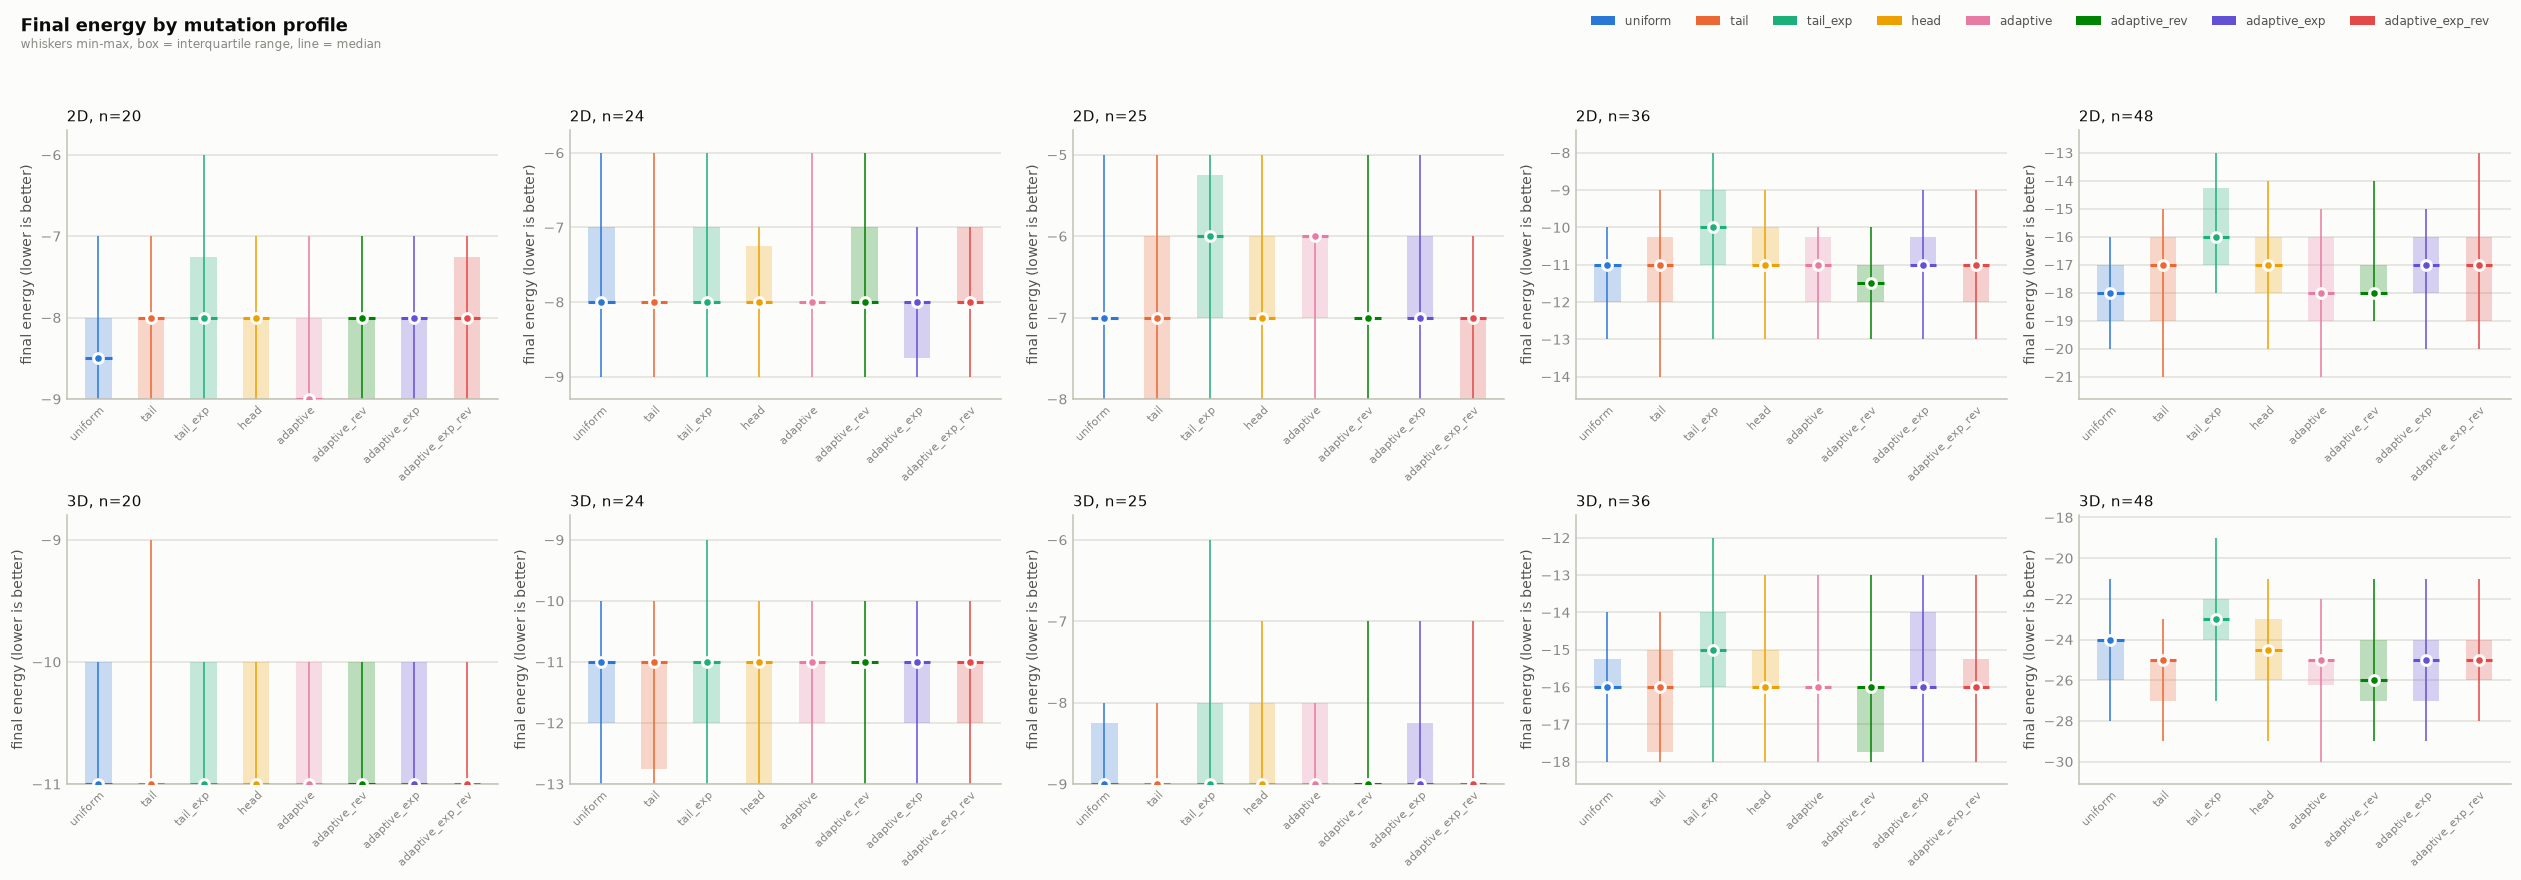
\includegraphics[width=0.97\linewidth]{../figures/final/energy.png}
\caption{A futások végső energiája profilonként (felül 2D, alul 3D, balról jobbra
a 20, 24, 25, 36 és 48 aminosavas lánc), ahol egy oszlop 30 futást ábrázol: a pont
a medián, a halvány téglalap a középső 50\%, a vékony vonal a legjobb és a
legrosszabb futás, és lefelé jobb az érték.}
\end{figure}

Az 1. ábra szerint a profilok végső energiája szinte mindenhol egyezik, az
eloszlások erősen átfednek. A 3D 20 és 25 aminosavas láncnál minden profil
mediánja a célenergián van ($-11$, illetve $-9$). A 24 aminosavas láncnál a
medián $-11$, két kapcsolattal a cél ($-13$) felett. A 2D rövid láncoknál a
medián egy kapcsolattal marad el a céltól. Egyetlen profil válik el a többitől:
a \texttt{tail\_exp} mediánja a hosszú láncoknál egy-két kapcsolattal rosszabb.
2D-ben ez szignifikáns (36 és 48 aminosav, Holm utáni $p\le 0{,}001$), 3D-ben nem
($p=0{,}13$, illetve $0{,}065$). A 48 aminosavas láncnál a 3D medián $-23$ és
$-26$ között van, a cél $-31$.
\end{landscape}

\begin{landscape}
\subsection{Kiértékelések a célig}

\begin{figure}[H]
\centering
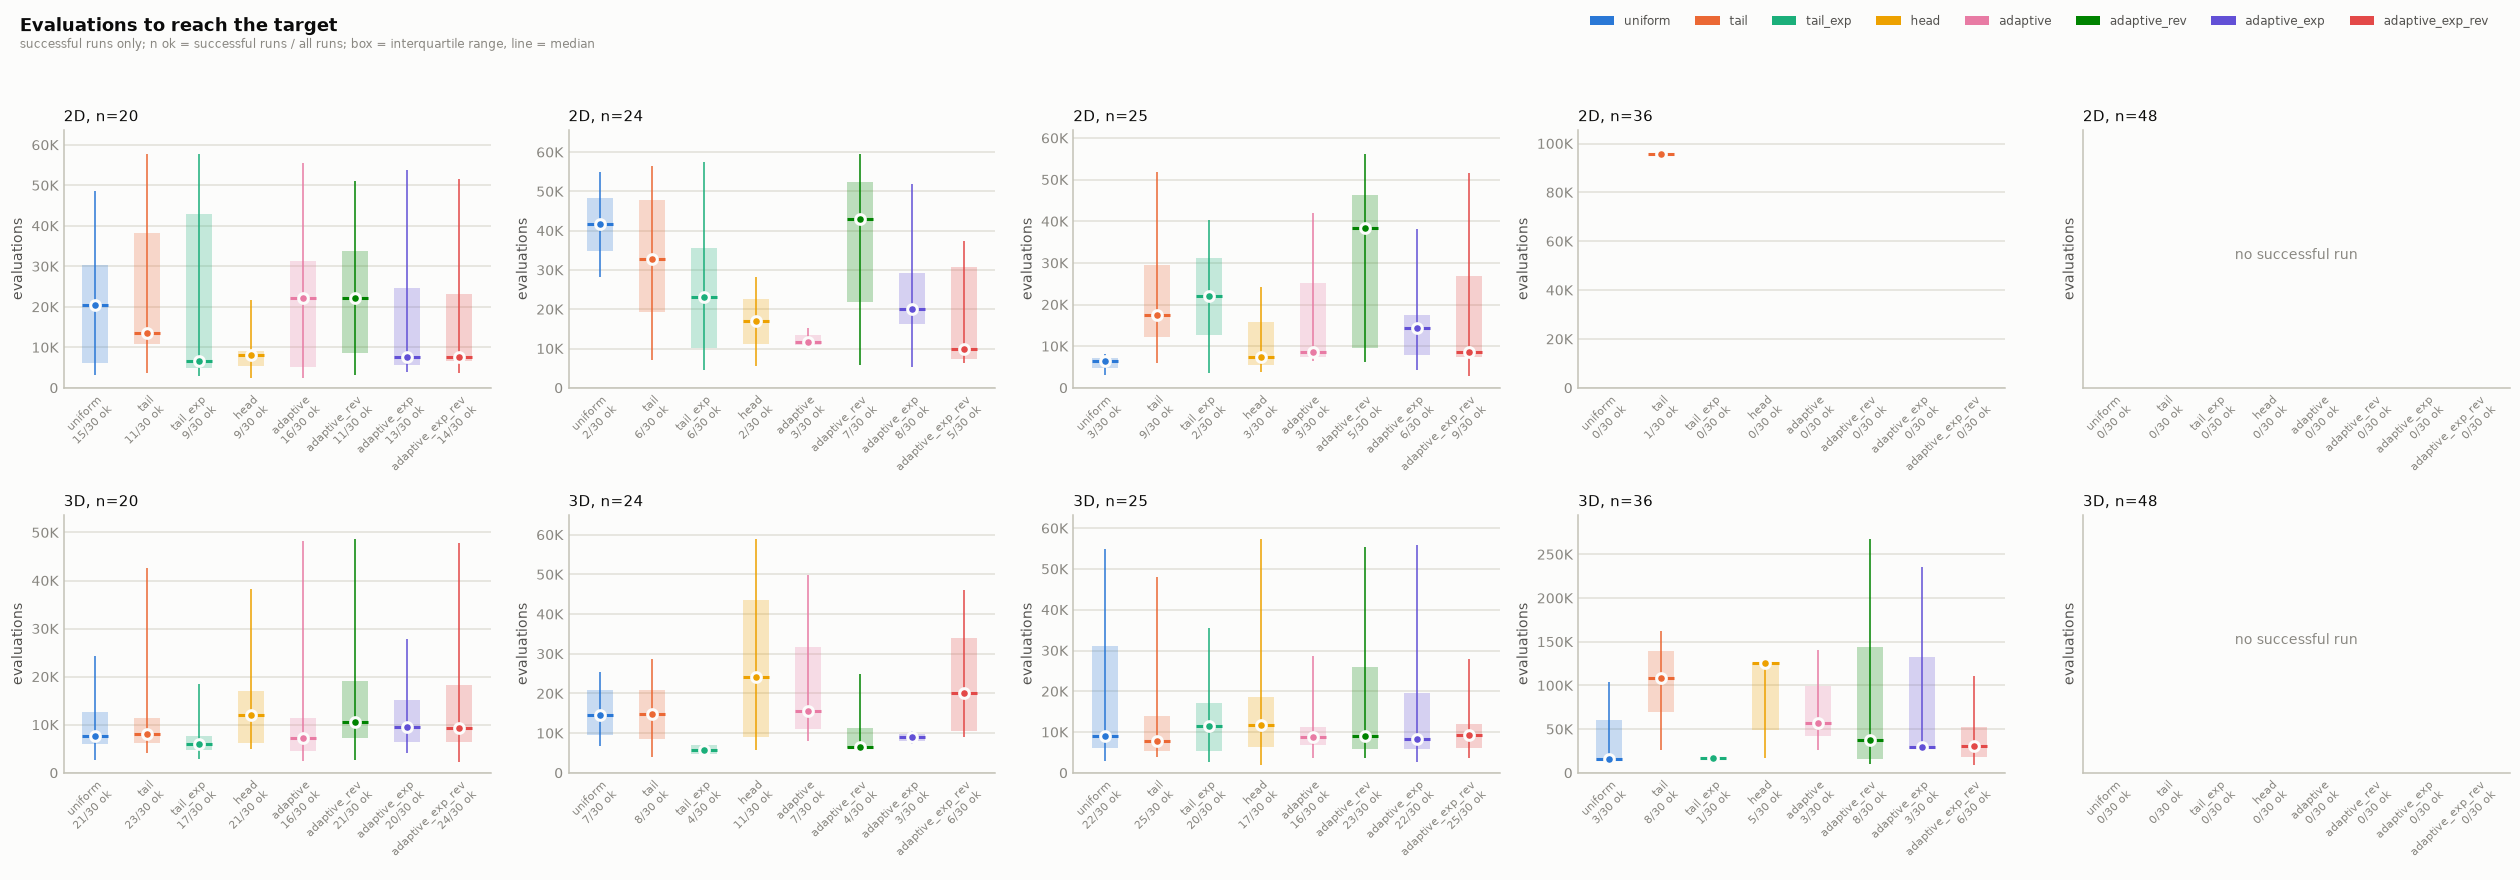
\includegraphics[width=0.97\linewidth]{../figures/final/evaluations.png}
\caption{A célenergia eléréséhez szükséges kiértékelések a sikeres futásokra, az
1. ábrával azonos jelöléssel és elrendezéssel, az oszlopok alatt a sikeres és az
összes futás számával.}
\end{figure}

A 2. ábra csak a sikeres futásokat tartalmazza, ezért az alacsony érték
félrevezető lehet, ha az oszlop alatt kevés futás áll: a lassú profil is
gyorsnak látszik, ha csak a szerencsés futásai szerepelnek. A 3D 20 és 25
aminosavas láncnál a sikeres futások mediánja 6000 és 12\,000 kiértékelés
között van, a profilok dobozai átfednek. A 3D 24 aminosavas láncnál a medián
6000 és 24\,000 között van, de a \texttt{tail\_exp} és az
\texttt{adaptive\_rev} oszlopa mindössze 4 sikeres futásra épül. A 3D 25
aminosavas láncnál a \texttt{tail} és az \texttt{adaptive\_exp\_rev} éri el
legtöbbször a célt (25/30), az egyenletes profil 22 alkalommal, a különbség
azonban nem szignifikáns. A 2D 36 és 48 aminosavas panel szinte üres, mert alig
volt sikeres futás.
\end{landscape}

\begin{landscape}
\subsection{Konvergencia}

\begin{figure}[H]
\centering
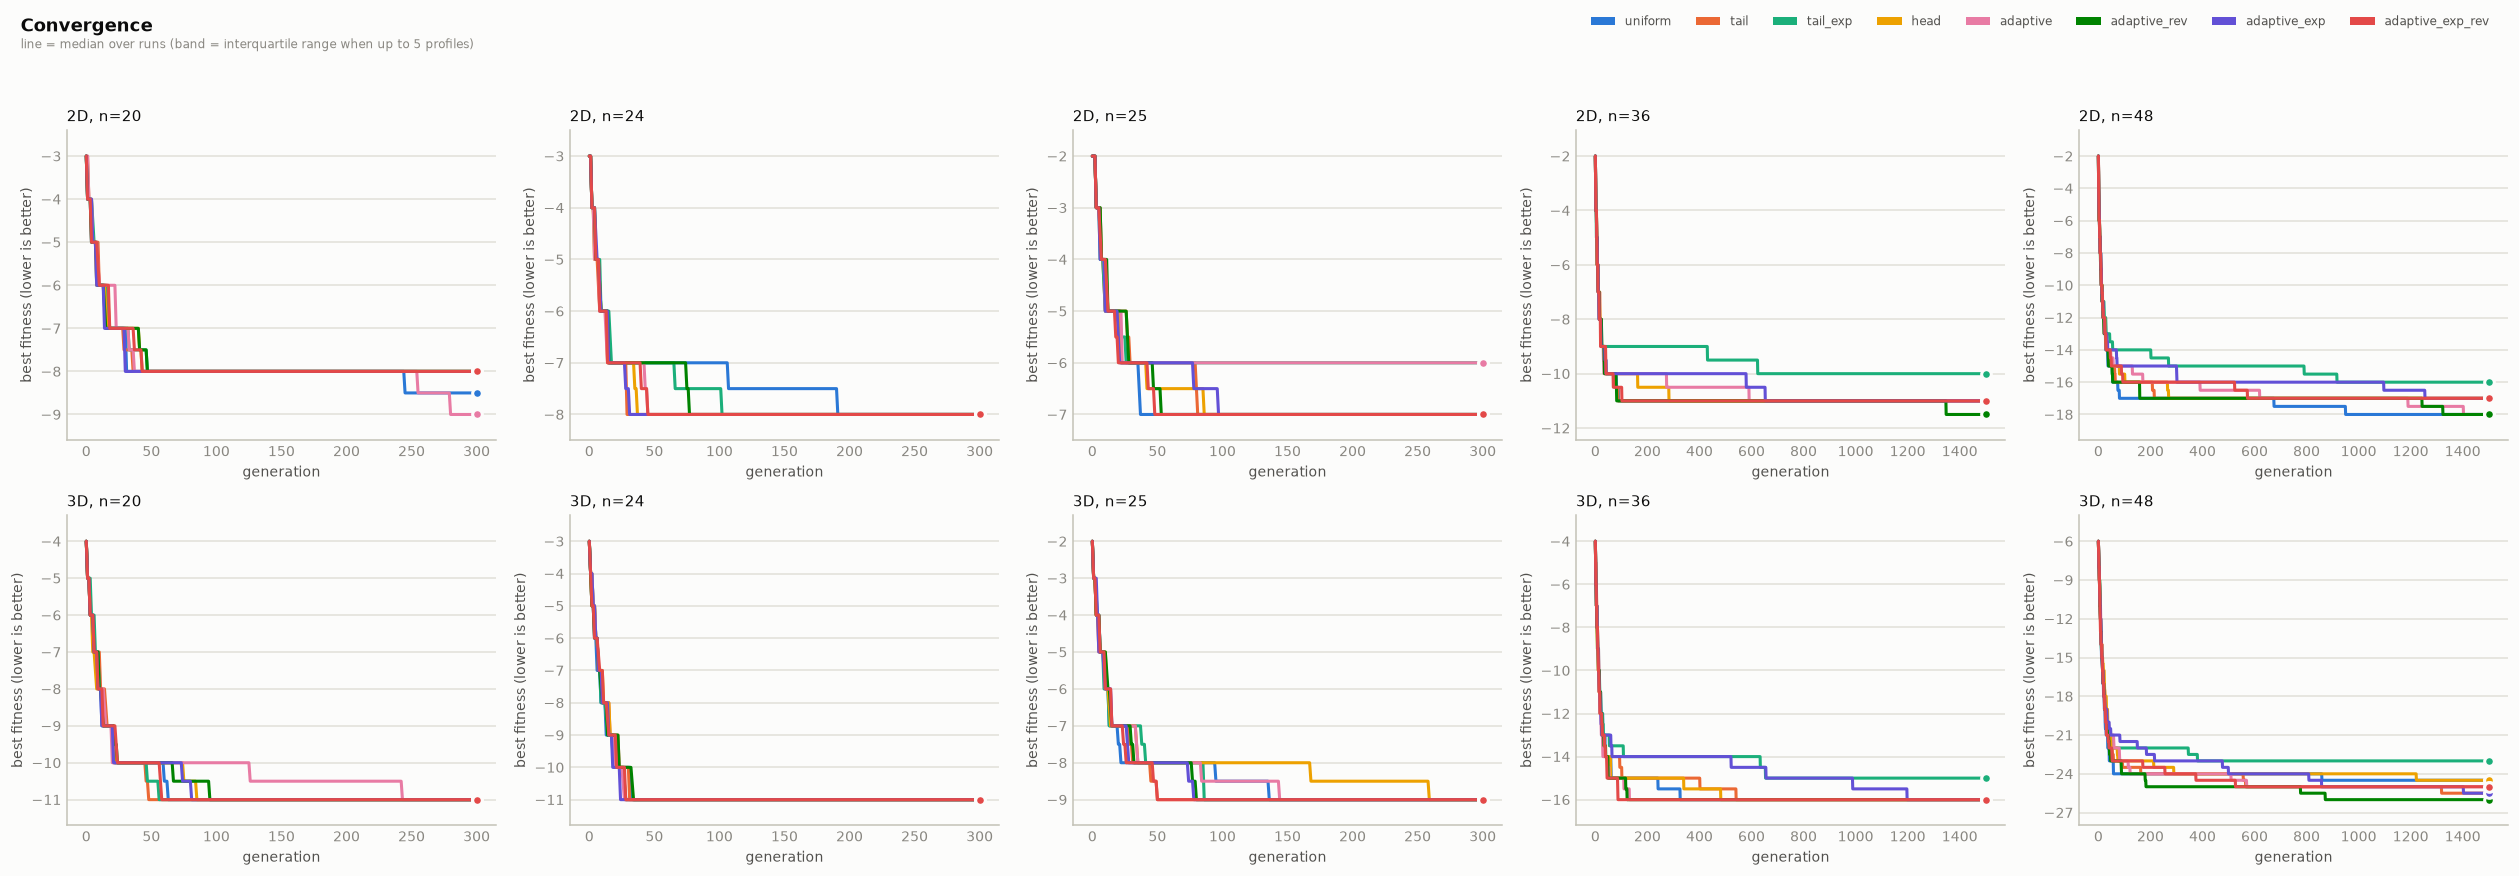
\includegraphics[width=0.97\linewidth]{../figures/final/curves.png}
\caption{A legjobb egyed fitnesze a generációk során, profilonként a 30 futás
mediánja (kisebb érték jobb).}
\end{figure}

A 3. ábra a futások menetét mutatja. Minden profil az első 100 generációban a
végső érték közelébe jut, utána a medián hosszú ideig vízszintes. A rövid
láncoknál a görbék gyakorlatilag egybeesnek, vagyis a mutáció helye a kezdeti
gyors javulást nem befolyásolja, legfeljebb az utolsó kapcsolat megtalálását. A
36 és 48 aminosavas láncnál a görbék jobban szétválnak, és 1000 generáció után is
előfordul javulás, ezért az 1500 generációs keret nem biztos, hogy elegendő.
\end{landscape}

\begin{landscape}
\subsection{A populáció változatossága}

\begin{figure}[H]
\centering
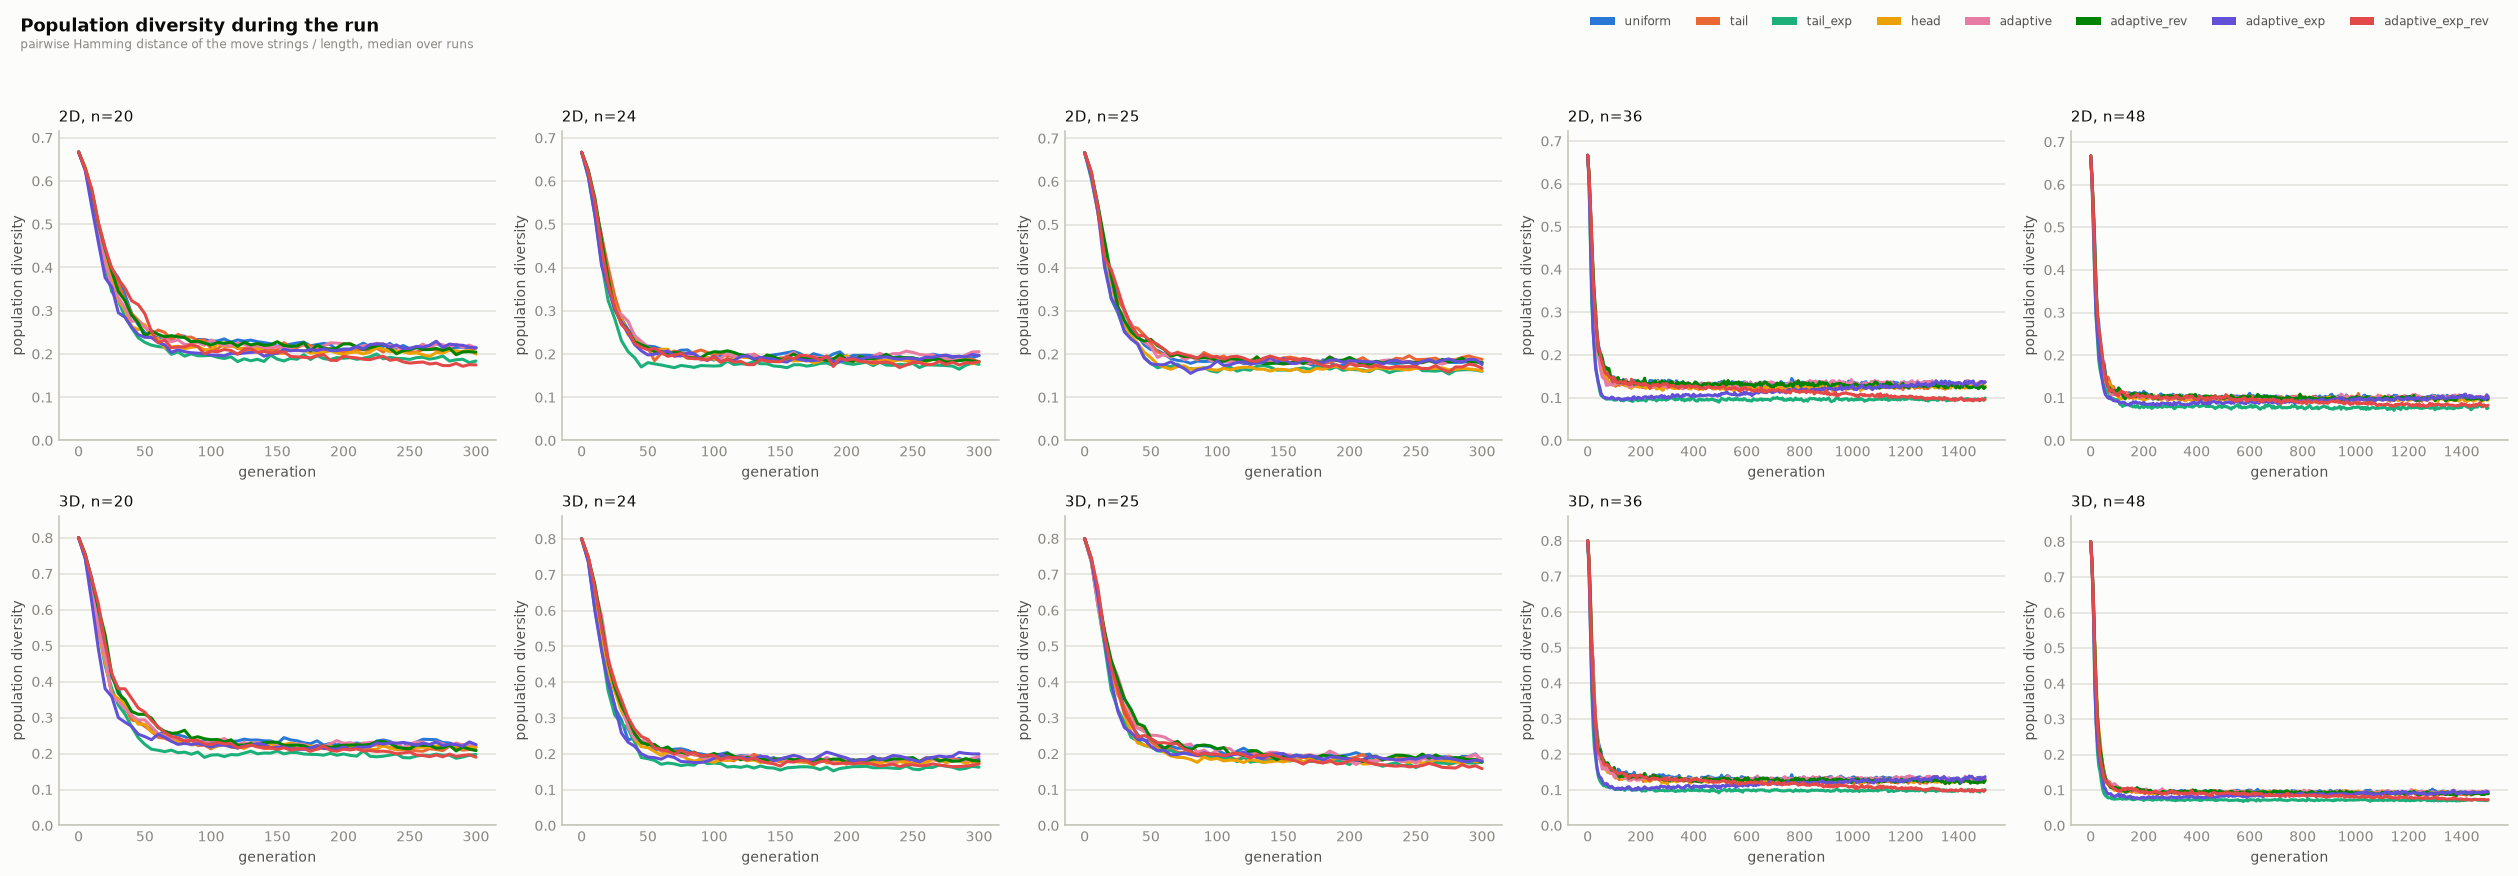
\includegraphics[width=0.97\linewidth]{../figures/diversity/over_time.png}
\caption{A populáció változatossága a generációk során (az átlagos páronkénti
Hamming-távolság a sztring hosszával osztva), profilonként a 30 futás mediánja, az
1. ábrával azonos elrendezésben.}
\end{figure}

A 4. ábra szerint a változatosság minden profilnál gyorsan csökken: a kezdeti 0,67
(2D), illetve 0,8 (3D) értékről az első 50 generációban 0,1 és 0,25 közé esik, 100
generáció után pedig alig változik. A rövid láncoknál a stabil érték 0,2 körüli, a 36 és
48 aminosavas láncnál 0,1 körüli. A populáció tehát ugyanabban az időszakban veszti
el változatosságának nagy részét, amikor a legjobb fitnesz is megáll (3. ábra). A
profilok görbéi nagyrészt egybeesnek, eltérést a meredek profilok mutatnak. A
\texttt{tail\_exp} futásátlagos változatossága mind a 10 cellában szignifikánsan
kisebb az egyenletesénél (Holm utáni $p<0{,}05$). A többi profil futásátlaga
kevesebb cellában tér el szignifikánsan, a \texttt{tail}-é csak a 36 aminosavas
láncnál. A különbségek a hosszú láncoknál
a legnagyobbak: a 3D 36 aminosavas láncnál a \texttt{tail\_exp} végső mediánja
0,10, az egyenleseé 0,13.
\end{landscape}

\subsection{2D és 3D összehasonlítása}

\begin{figure}[H]
\centering
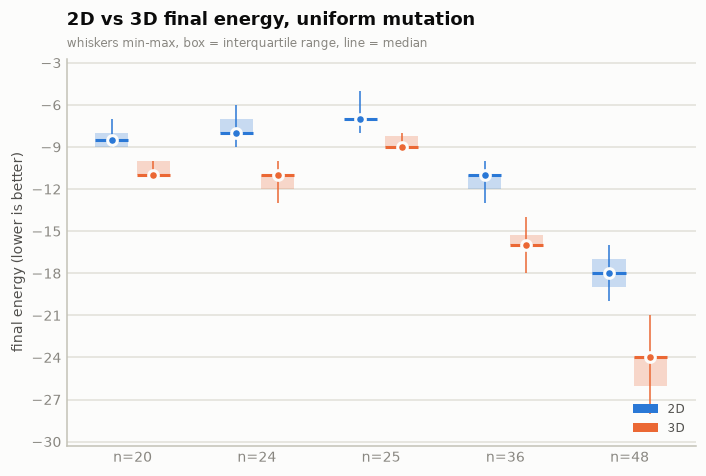
\includegraphics[width=0.62\linewidth]{../figures/final/dimension.png}
\caption{A végső energia 2D-ben (kék) és 3D-ben (narancs) egyenletes mutációval,
az 1. ábrával azonos jelöléssel.}
\end{figure}

Az 5. ábra szerint a 3D medián minden szekvenciánál kisebb. A különbség 2,5; 3; 2; 5
és 6 kapcsolat a 20, 24, 25, 36 és 48 aminosavas láncnál, a hosszú láncoknál
tehát nagyobb. A dobozok sehol nem fedik egymást.

\subsection{A hipotézisek értékelése}

\begin{table}[H]
\centering
\small
\begin{tabular}{p{0.05\linewidth}p{0.30\linewidth}p{0.55\linewidth}}
\toprule
 & Várt & Kapott \\
\midrule
H1 & \texttt{tail} és \texttt{tail\_exp} kevesebb kiértékelés, nem rosszabb energia & Nem igazolt. 20 próbából 1 nyers $p<0{,}05$ (2D, $n=25$, \texttt{tail}, $p=0{,}049$), Holm után 0. A \texttt{tail} a 10 cellából 7-ben több sikert ad, 1-ben kevesebbet, 2-ben egyik sem sikeres. A \texttt{tail\_exp} rosszabb. \\
H2 & \texttt{head} rosszabb, mint \texttt{uniform} & Nem igazolt. 10 próbából 0 szignifikáns. A \texttt{head} összesen 68 sikert ad, az egyenletes 73-at. \\
H3 & Az adaptív nem rosszabb a legjobb fixnél & Nem cáfolt. 40 próbából 4 nyers $p<0{,}05$ az adaptív kárára, Holm után 0. Egyik adaptív profil sem szignifikánsan jobb az egyenletesnél. \\
H4 & 3D energiája kisebb & Igazolt. 40 próbából 40 szignifikáns Holm után is. \\
\bottomrule
\end{tabular}
\caption{Várt és kapott eredmények hipotézisenként. Minden próba egyoldali
Mann-Whitney-próba, Holm-korrekcióval hipotézisenként.}
\end{table}

A H3 próbájánál a legjobb fix profilt ugyanazokon az adatokon választottuk, a
legkisebb ERT alapján, ezért a próba szigorúbb az adaptív profilokkal szemben. A
négy nyers szignifikáns eset egyike sem marad meg a Holm-korrekció után.

\subsection{Feltáró vizsgálat: a változatosság növelése}

A változatosság gyors elvesztése miatt két egyszerű beavatkozást próbáltunk ki.
Hipotézist nem fogalmaztunk meg hozzájuk, az eredményeket feltáró jelleggel
közöljük. Az egyik az átlagos mutációs ráta 2, 4, illetve 8-szorosára emelése
(\texttt{rate2}, \texttt{rate4}, \texttt{rate8}). A másiknál az új generáció 5, 10,
illetve 20\%-a véletlen új egyed (\texttt{imm5}, \texttt{imm10}, \texttt{imm20}),
az elit egyedek változatlanul megmaradnak. Az új egyedeket is ki kell értékelni,
ezért minden változat generációnként ugyanannyi kiértékelést használ, mint az
alapváltozat. A mérés egyenletes profillal, a 3D 24 és 36 aminosavas láncon, 30
maggal és a végső mérés céljaival és kereteivel készült. A \texttt{base} sor a
végső mérés egyenletes profiljával azonos. A változatokat az alapváltozattal
hasonlítottuk össze, a 12 összehasonlításon Holm-korrekcióval.

\begin{table}[H]
\centering
\small
\setlength{\tabcolsep}{4pt}
\begin{tabular}{lrrrrrrrr}
\hline
& \multicolumn{4}{c}{3D 24} & \multicolumn{4}{c}{3D 36} \\
változat & siker & ERT & energia & vált. & siker & ERT & energia & vált. \\
\hline
\texttt{base} & 7 & 211 & \textbf{$-11$} & 0,24 & 3 & 2719 & \textbf{$-16$} & 0,15 \\
\texttt{rate2} & 1 & 1744 & \textbf{$-11$} & 0,59 & 4 & 2050 & \textbf{$-16$} & 0,48 \\
\texttt{rate4} & 0 & nincs & $-8$ & 0,77 & 0 & nincs & $-13$ & 0,74 \\
\texttt{rate8} & 0 & nincs & $-7$ & 0,80 & 0 & nincs & $-11$ & 0,79 \\
\texttt{imm5} & \textbf{8} & \textbf{180} & \textbf{$-11$} & 0,33 & 4 & 2094 & \textbf{$-16$} & 0,23 \\
\texttt{imm10} & \textbf{8} & 189 & \textbf{$-11$} & 0,40 & 8 & 906 & \textbf{$-16$} & 0,32 \\
\texttt{imm20} & 7 & 234 & \textbf{$-11$} & 0,54 & \textbf{9} & \textbf{765} & \textbf{$-16$} & 0,48 \\
\hline
\end{tabular}

\caption{A változatosság növelésére kipróbált változatok. Siker: a célt elérő futások
száma 30-ból. ERT: ezer kiértékelésben. Energia: a végső energia mediánja. Vált.: a
futás egészére átlagolt változatosság mediánja, amelyben az új egyedek is
szerepelnek. Félkövér: a legjobb érték oszloponként.}
\label{tab:remedies}
\end{table}

A mutációs ráta növelése rontott az eredményen. A kétszeres ráta a 24 aminosavas
láncon 7-ről 1-re csökkentette a sikeres futások számát (nyers $p=0{,}052$, Holm
után nem szignifikáns), a négy- és a nyolcszoros ráta mellett pedig egyik futás sem
érte el a célt. Mindkét láncon a végső energia ekkor szignifikánsan rosszabb (Holm
utáni $p<0{,}001$). A változatosság 0,6 és 0,8 közé emelkedik, vagyis a populáció a
véletlen szint (0,8) közelében marad, és nem hajtogat jobban.

A véletlen új egyedek a 24 aminosavas láncon nem változtatnak az eredményen (7 helyett
7 vagy 8 siker). A 36 aminosavas láncon az új egyedek arányával nő a sikeres futások
száma (3, 4, 8, illetve 9), és csökken az ERT (2,7 millióról 2,1; 0,9, illetve 0,77
millióra). A legnagyobb eltérésnél (\texttt{imm20}) a nyers $p$ a kiértékelésekre
0,076, a sikerekre 0,10, Holm után egyik sem szignifikáns, a végső energia pedig nem
változik. Az irány tehát egyezik azzal, hogy a változatosság hiánya lassítja a
keresést, de 30 futással ez nem erősíthető meg.

\section{Megbeszélés}

\paragraph{Fő kérdés.} A mutáció helye alig számít. 30 futásnál a profilok között
nincs olyan eltérés a kiértékelésekben vagy a sikerekben, amely a Holm-korrekciót
kibírná. Az egyetlen megerősített hatás, hogy a túl meredek \texttt{tail\_exp}
rontja a végső energiát a 2D hosszú láncokon. A \texttt{tail} adja a legtöbb
sikert (91 az egyenletes 73-ával szemben), de ez az előny egyetlen cellában sem
szignifikáns, és nagyobb mintával dönthető el. Az adaptív változatok nem
múlják felül a fix profilokat.

A konvergenciagörbék szerint a legjobb egyed gyorsan eléri a végső érték közelét,
utána a futás megreked. Ugyanebben az időszakban esik a populáció változatossága a
kezdeti érték harmadára vagy kisebbre, ezért a megrekedés összefügghet a
változatosság elvesztésével. A legkevésbé változatos profil, a \texttt{tail\_exp}
az egyetlen, amelynek végső energiája a 2D hosszú láncokon megerősítetten
rosszabb. Ez nem ok-okozati bizonyíték. A feltáró mérésben a véletlen új egyedek a
36 aminosavas láncon kevesebb kiértékelést igényeltek, de ez nem szignifikáns, ezért
a változatosság szerepét nem döntötte el. A mutációs ráta emelése ugyanakkor nem
helyettesíti a változatosságot: a túl nagy ráta véletlen kereséssé alakítja a GA-t.

\paragraph{Másodlagos kérdés.} A 3D változat valóban több H-H kapcsolatot ér el, és
a különbség a hosszú láncoknál nagyobb.

\paragraph{Korlátok.}
\begin{itemize}
\item A 36 és 48 aminosavas célok, valamint a 2D célok az irodalomban ismert
legjobb értékek, nem bizonyított optimumok. A 48 aminosavas láncot egyetlen futás
sem oldotta meg, ezért itt az ERT nem értelmezhető, és csak az energiákat
hasonlíthatjuk össze.
\item Egy cellában 30 futás van, ezért csak nagy eltérés válik szignifikánssá. A
korrekció több száz összehasonlításra szigorú.
\item Az exponenciális alapot és a hosszú szekvenciák keretét előzetes mérés
alapján választottuk. A három újabb adaptív profil a hipotézisek rögzítése után került
a vizsgálatba, ezért az ezekre vonatkozó eredmények feltáró jellegűek.
\item A változatosságot csak a lépéssorozatok szintjén mértük, a hajtogatások
alakjának változatosságát nem.
\item A GA többi beállításának (populáció, keresztezés, elitizmus) hatását nem
mértük.
\end{itemize}

\paragraph{További irány.} A GA a rövid láncokat megoldja, a hosszúakat nem.
Ezekre a memetikus változat, amelyben a GA minden utódját rövid helyi keresés
követi, javulást hozhat. Ennek vizsgálata külön hipotézist és külön mérést
igényel.

\clearpage
\section{Reprodukálhatóság}

A teljes kód a \texttt{src/} mappában található. Python 3 szükséges, a használt
csomagok a numpy, a scipy, a matplotlib és a pillow, pontos verzióik a
\texttt{requirements.txt} fájlban szerepelnek. A véletlen magok 0 és 29 között
vannak. Azonos mag azonos futást ad,
a párhuzamos végrehajtás nem változtatja meg az eredményt. A teljes mérés 9
processzen 54 percig tart, a változatossági mérés 51 percig. A projekt gyökeréből:
\begin{verbatim}
.venv/bin/python src/test_hp.py
cc -O2 -o exact_3d src/exact_3d.c
.venv/bin/python src/run_experiment.py --seeds 30 \
  --out results/final.csv --workers 9
.venv/bin/python src/hp_stats.py results/final.csv
.venv/bin/python src/hp_plots.py results results/final.csv
.venv/bin/python src/hp_diversity.py run --seeds 30 \
  --out results/diversity.csv --workers 9
.venv/bin/python src/hp_diversity.py stats results/diversity.csv
.venv/bin/python src/hp_plots.py diversity results/diversity.csv
.venv/bin/python src/hp_remedies.py run --seeds 30 \
  --out results/remedies.csv --workers 9
.venv/bin/python src/hp_remedies.py stats results/remedies.csv
.venv/bin/python src/hp_fold3d.py videos
\end{verbatim}
A \texttt{videos/} mappa a GA egy-egy futását mutatja szekvenciánként és
rácsonként (egyenletes profil, 0. mag), a célenergiával együtt. A 3D optimumokat a
\texttt{./exact\_3d SEQ X Y Z Emin} parancs igazolja (szekvencia, a doboz mérete,
a H-mag legkisebb kapcsolatszáma).

\end{document}
